\documentclass[10pt]{exam}
\usepackage[hon]{template-for-exam}
\usepackage{graphicx}
\usepackage{caption,multicol,tikz}
\usepackage{silence}
\WarningFilter{latex}{Label `question}
\WarningFilter{latex}{There were multiply-defined labels}
\usetikzlibrary{decorations.markings}

\title{Refraction Lab}
\author{Rohrbach}
\date{\today}

\begin{document}
\maketitle

\noindent
{\small \it This lab is based on Experiment \#4 in PASCO's Introductory Optics System Manual and the first illustration is borrowed from it.}


\section*{Pre-Lab}

Read the following pages in your book and answer these questions:

\begin{questions}
\uplevel{\subsection*{Geometric Optics, The Ray Model of Light, and Reflection (pp. 644-645)}}

  \question What does light have to do with electricity and magnetism? \vs
  \question What is the \emph{Ray Model of Light}? \vs
  \question How is the angle of incidence and angle of reflection measured? \vs
  \question What is the \emph{Law of Reflection}? \vs  

\uplevel{\subsection*{Refraction and Index of Refraction (pp. 656-657)}}

  \question What is \emph{index of refraction}? \vs
  \question What are the units of index of refraction? \vs
  \question What is \emph{refraction}? \vs 
  \question When does light bend toward and away from normal? \vs 


\end{questions}

\pagebreak

\section*{Purpose} To observe what happens to rays of light refract at a lens

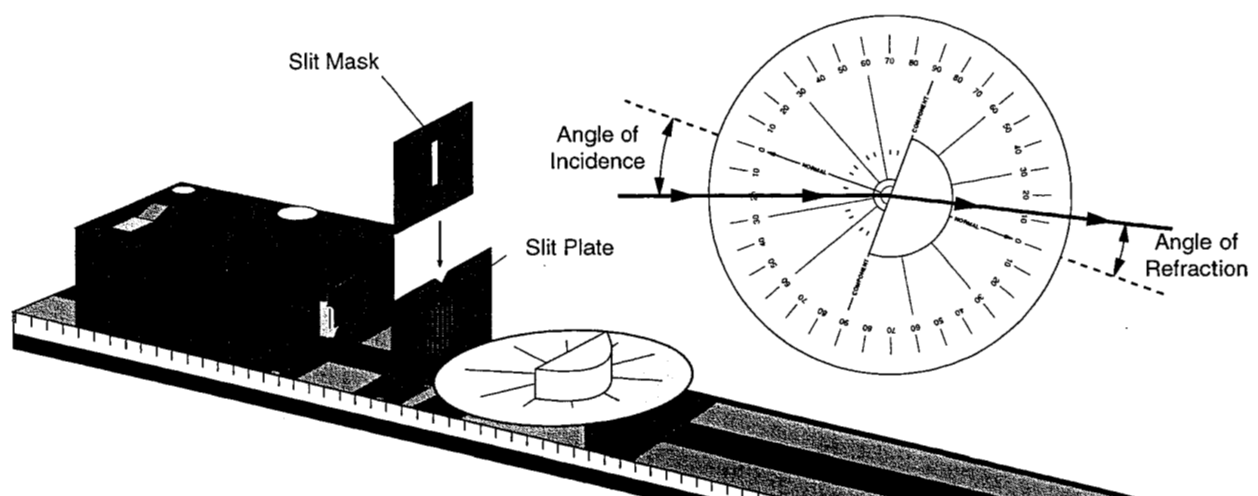
\includegraphics[width=15cm]{Fig4_1.png}

\vspace{-1em}

\section*{Procedure}
\begin{enumerate}
  \item Set up the experiment as indicated above.
  \item Adjust the components so that a single ray of light is aligned with the bold arrow labeled ``normal'' on the Ray Table Degree Scale.
  \item Carefully align the flat part of the Cylindrical Lens along the bold arrow labeled ``component'' on the Ray Table Degree Scale.  Adjust the placement of the lens so that the angle of refraction is $0^\circ$.  From this point forward, be careful when adjusting the Ray Table so that the lens does not slip.
  \item Rotate the Ray Table so that the Angle of Incidence changes.  Record the angle of refraction and the angle of reflection.
  \item We will need to take data for both {\bf Air $\rightarrow$ Glass} Refraction and {\bf Glass $\rightarrow$ Air} Refraction.  Label each situation and label the incident, reflected, and refracted ray. 
  
  \begin{center}
    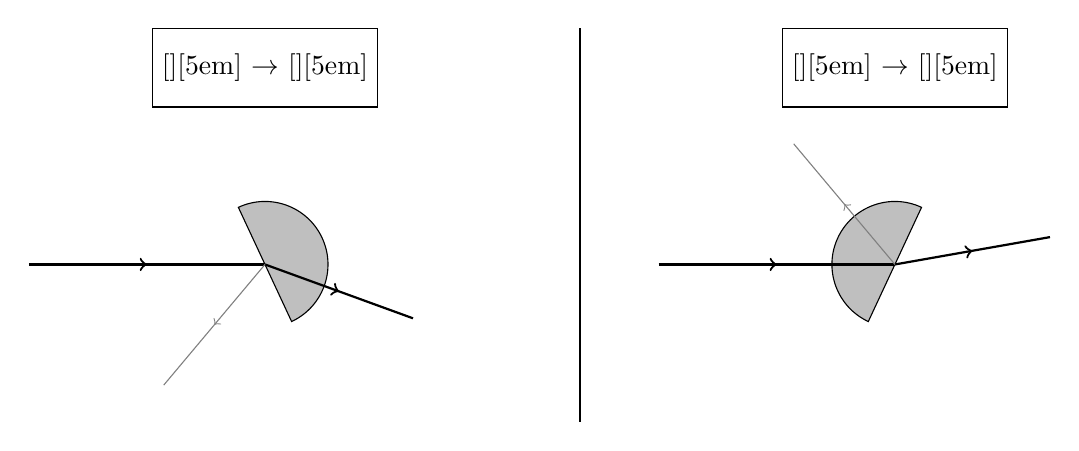
\begin{tikzpicture}[decoration={
      markings,
      mark=at position 0.5 with {\arrow{>}}
    }]
      \draw (0,3) -- (0,-2);
  
      \begin{scope}[shift={(-4,0)}]

        \node[draw, minimum height=1cm] at (0,2.5) {\fillin[][5em] $\rightarrow$ \fillin[][5em]};
  
        \begin{scope}[rotate=-65]
          \draw[fill=gray!50] (-0.8,0) arc (180:0:0.8) -- cycle;
        \end{scope}  
  
        \draw[thick, postaction={decorate}] 
          (-3,0)-- (0,0);\draw[thick, postaction={decorate}] 
          (0,0) -- (-20:2);
        \draw[black!50,postaction={decorate}] 
          (0,0) -- ++(-130:2); 
  
      \end{scope}
  
      \begin{scope}[shift={(4,0)}]
        \node[draw, minimum height=1cm] at (0,2.5) {\fillin[][5em] $\rightarrow$ \fillin[][5em]};

        \begin{scope}[rotate=65]
          \draw[fill=gray!50] (-0.8,0) arc (180:0:0.8) -- cycle;
        \end{scope}  
  
        \draw[thick, postaction={decorate}] 
          (-3,0)-- (0,0);\draw[thick, postaction={decorate}] 
          (0,0) -- (10:2);
        \draw[black!50,postaction={decorate}] 
          (0,0) -- ++(130:2); 
      \end{scope}
  
  
    \end{tikzpicture}
  \end{center}
  
\end{enumerate}




\pagebreak

\section*{Data}

\emph{Not all of the rays will be visible.  If a ray is not visible, write ``{\bf n.v.}'' for ``not visible.''}

\renewcommand{\arraystretch}{1.7}

\begin{multicols}{2}
  \begin{tabular}{|c|c|c|}
    \hline
    \multicolumn{3}{|c|}{Angles for {\bf Air $\rightarrow$ Glass}} 
    \\\hline
    Incidence &
    Refraction &
    Reflection \\\hline
    $10^\circ$ && \\\hline
    $20^\circ$ && \\\hline
    $30^\circ$ && \\\hline
    $40^\circ$ && \\\hline
    $50^\circ$ && \\\hline
    $60^\circ$ && \\\hline
    $70^\circ$ && \\\hline
    $80^\circ$ && \\\hline
  \end{tabular}

  \columnbreak

  \begin{tabular}{|c|c|c|}
    \hline
    \multicolumn{3}{|c|}{Angles for {\bf Glass $\rightarrow$ Air}} 
    \\\hline
    Incidence &
    Refraction &
    Reflection \\\hline
    $10^\circ$ && \\\hline
    $20^\circ$ && \\\hline
    $30^\circ$ && \\\hline
    $40^\circ$ && \\\hline
    $50^\circ$ && \\\hline
    $60^\circ$ && \\\hline
    $70^\circ$ && \\\hline
    $80^\circ$ && \\\hline
  \end{tabular}


\end{multicols}

\vspace{-1em}
\begin{questions}

\uplevel{\section*{Analysis}}

  \question
    Take a look at how the light bends.  It only bends at the flat surface; it does not bend at the curved surface of the lens.  Why do you suppose this is? 
    \vs 

  \question
    The results of the two trials ({\bf Air $\rightarrow$ Glass} and {\bf Glass $\rightarrow$ Air}) are not the same.  What pattern do you notice with the angles of refraction? (\emph{i.e.} Are they larger or smaller than the angle of incidence?)
    \vs
  
  \question
    What difficulties did you have at large angles?  Why do you think these difficulties arose?
    \vs 
  
  \question
    What did you notice about the angle of reFLECtion?
    \vs 



\end{questions}

\pagebreak

\vfill\,




\end{document}